%!TEX root = ../tesis.tex
\chapter{Soluci\'on Propuesta}
\label{sec:solucion}

Numerosas aplicaciones en el \'area del reconocimiento del habla han sido desarrolladas: 
\emph{Siri} \cite{AppleSiri}, \emph{Google Now} \cite{GoogleNow}, 
\emph{Dragon Naturally Speaking} \cite{DragonNaturallySpeaking}, etc. Cada una de estas
aplicaciones satisface distintos tipos de requerimientos pensados o inspirados en las necesidades de los usuarios finales. 

En el cap\'itulo anterior se presentó el desafío que supone el diseño de interfaces basadas 
en reconocimiento del habla, así como los requerimientos básicos de la aplicación a ser implementada como 
parte de este trabajo.

Este cap\'itulo presenta, justifica y describe la soluci\'on espec\'ifica al problema de implementar 
una interfaz basada en reconocimiento del habla para la aplicaci\'on escogida.


%!TEX root = ../tesis.tex

\section{Aplicaci\'on Desarrollada}
\label{sec:aplicacion-desarrollada}

Como se expone en la secci\'on~\ref{sec:problema-especifico}, se propone el dise\~no
de una interfaz para componer m\'usica utilizando la voz. Adem\'as, este trabajo 
opta por la metodolog\'ia de trabajo de c\'odigo abierto, lo cual implica: 

\begin{itemize}
    \item Utilizar tecnolog\'ias de c\'odigo abierto para el desarrollo de la interfaz.
    \item Establecer un proceso de desarrollo transparente y abierto.
\end{itemize}

La metodolog\'ia adoptada para implementar la interfaz permite utilizar un proyecto
existente como punto de partida, y as\'i dise\~nar e implementar una interfaz alternativa que permite
controlar la aplicaci\'on por comandos de voz. Adem\'as,
el hecho de incorporar una nueva interfaz, permite analizar
una de las motivaciones de la secci\'on~\ref{sec:motivacion}: un programa de composici\'on
musical, que recibe comandos sonoros y emite tambi\'en un resultado sonoro, podr\'ia ser
m\'as natural para el usuario. 

La interfaz desarrollada se denomina \emph{TamTam Listens} y toma como punto de partida la 
aplicaci\'on \emph{TamTam Edit} de la plataforma educativa \foreign{Sugar}.

\subsection{TamTam Edit}
\label{sec:tamtam-edit}

La m\'usica es a menudo descrita como la forma m\'as pura de representaci\'on matem\'atica, es m\'as,
te\'oricos de la m\'usica han utilizado las matem\'aticas para resolver problemas musicales
\cite{TheSoundOfNumbers}. Esta fue la inspiraci\'on para la creaci\'on del compendio de 
actividades\footnote{Una Actividad, es una aplicaci\'on en el entorno de escritorio \emph{Sugar}.}
conocido como \emph{TamTam} desarrollado para la computadora XO\footnote{La XO, es una computadora 
port\'atil de bajo costo y consumo desarrollada por el proyecto \gls{olpc}.},
con los siguientes objetivos:

\begin{itemize}
    \item Proveer a los ni\~nos un ambiente de informaci\'on cultural construyendo m\'usica y sonidos.
    \item Brindar una experiencia sonora/musical divertida para usuarios sin conocimientos musicales.
    \item Promover un camino hacia experiencias musicales m\'as sofisticadas.
    \item Promover un instrumento musical con su propio ``sonido''.
    \item Desarrollar un ambiente din\'amico y mutable que propone la simpleza y permite la complejidad.
    \item Favorecer la creaci\'on de m\'usica grupalmente.
    \item Introducir los conceptos musicales y otros como: programaci\'on y audio.
\end{itemize}

\emph{TamTam Edit} es una aplicaci\'on, parte del conjunto de actividades musicales 
\emph{TamTam}, que proporciona una interfaz intuitiva para crear, modificar y organizar notas ubicadas 
en pistas virtuales.
Adem\'as incluye una paleta de casi cien tipos de sonidos y modelos de construcci\'on musical que permite 
crear distintos tipos de variaciones en estilos musicales \cite{TamTamWiki}.


Las secciones principales del programa se pueden observar en la figura~\ref{figure:ui-tamtam} 

\begin{figure}[H]
\centering
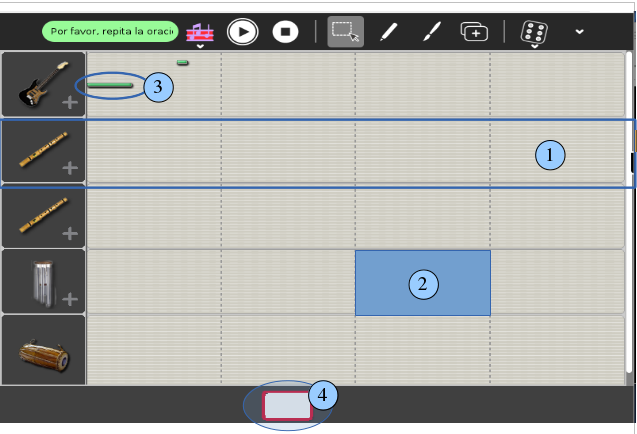
\includegraphics[width=0.8\textwidth]{./graphics/ui-tamtam-edit.png}
\caption{Interfaz de \emph{Tamtam Edit} y sus secciones principales.}
\label{figure:ui-tamtam}
\end{figure}

Como se puede apreciar en la figura~\ref{figure:ui-tamtam}, la interfaz se encuentra organizada en 
cinco pistas y cada pista (1) tiene asociada un instrumento (la quinta pista esta reservada para
instrumentos de tipo bater{\'\i}a). Cada pista se divide en 4 
compases (del comp\'as uno al cuatro) y cada comp\'as (2) se divide en 12 tiempos (del uno al doce). 
Las notas (3) se dibujan en los compases, como se puede ver, la longitud de la nota indica su 
duraci\'on y su altura el tipo de nota. Adem\'as la aplicaci\'on esta organizada en partituras (4), que 
son como hojas de cuaderno, y son \'utiles para componer m\'usicas largas.

En general, la interacci\'on entre el usuario y \foreign{TamTam Edit} que se presenta en
la figura~\ref{figure:ui-tamtam} se realiza de modo tradicional.
El usuario utiliza el teclado y el rat\'on para interactuar con la aplicaci\'on a trav\'es de elementos
gr\'aficos como botones y men\'us. 

Este trabajo de grado busca incorporar un medio de interacci\'on alternativo al propuesto 
por \emph{TamTam Edit}. A continuaci\'on se presentan los motivos que determinaron la elecci\'on 
de esta aplicaci\'on como punto de partida:

\begin{itemize}
    \item Impacto social: \emph{TamTam Edit} es una aplicaci\'on que forma parte de la plataforma establecida
    por el proyecto \gls{olpc}, el cual busca potenciar el proceso educativo \cite{OLPC}. 
    Los ni\~nos con alg\'un tipo de discapacidad tienen a menudo problemas para utilizar una computadora mediante
    dispositivos perif\'ericos tradicionales como el mouse o el teclado.

    En estos casos, la posibilidad de operar esta actividad mediante la voz ser{\'\i}a de gran beneficio 
    para los ni\~nos, mejorando la accesibilidad de la plataforma, y generando por tanto un impacto social
    positivo importante.
    \item Naturalidad de interacci\'on: utilizar la voz para interactuar con una aplicaci\'on podr{\'\i}a
    ofrecer una mayor naturalidad con respecto al enfoque tradicional de interacci\'on, teniendo en cuenta
    que es el medio de interacci\'on entre las personas.
    \item No reinventar la rueda: como el objetivo es incorporar una interfaz basada en reconocimiento del
    habla a una aplicaci\'on, se elige \emph{TamTam Edit} para no construir la aplicaci\'on desde cero,
    sino extender las capacidades de una ya existente.
    \item C\'odigo abierto: el motivo anterior es posible gracias a que \emph{TamTam Edit} es un 
    proyecto de c\'odigo abierto, lo cual brinda a los desarrolladores la libertad de extender las 
    funcionalidades de la aplicaci\'on.
    \item Lenguaje de programaci\'on: la actividad se encuentra implementada en el lenguaje de 
    programaci\'on Python. La librer{\'\i}a de reconocimiento del habla a ser utilizada proporociona 
    \emph{bindings} 
    \footnote{Un \emph{binding} es un componente \emph{software}
   que permite hacer uso de las funcionalidades prove{\'\i}das por una librer{\'\i}a, implementada
    en un determinado lenguaje de programaci\'on, utilizando un lenguaje de programaci\'on diferente. 
    En este caso particular, \emph{Pocketsphinx} est\'a implementado en C y C++.} para 
    este lenguaje, lo cual supone una ventaja importante para la implementaci\'on de la interfaz.
\end{itemize}

\subsection{Tamtam Listens}
\label{sec:tamtam-listens}

La interfaz de interacci\'on alternativa para la aplicaci\'on \emph{Tamtam Edit} se denomina  
\emph{Tamtam Listens}. \emph{Tamtam Listens} permite al usuario componer m\'usica utilizando comandos
de voz para acceder a las diferentes funcionalidades ofrecidas por \mbox{\emph{Tamtam Edit}.}

Al ofrecer al usuario final un medio de interacci\'on humano-computadora diferente, \emph{TamTam Listens}
debe ser intuitivo y f\'acil de usar. De modo a lograr esto, la soluci\'on a implementar no debe 
ofrecer al usuario la posibilidad de controlar el \foreign{mouse} o los componentes de la interfaz 
gr\'afica de \emph{TamTam Edit} utilizando la voz. 

Una correspondencia directa entre los comandos de voz y la interfaz gr\'afica puede resultar en 
un flujo de interacci\'on poco natural e inadecuado, motivado \'unicamente por la intenci\'on err\'onea 
de imitar el flujo de interacci\'on de las interfaces de escritorio tradicionales. 
La necesidad de ofrecer un flujo de interacci\'on diferente y apropiado para una interfaz mediante voz
como parte de \emph{TamTam Listens} se hizo clara durante la fase de dise\~no.

Para comprender la diferencia, puede considerarse el siguiente ejemplo. 
Crear una nota exige una secuencia de operaciones con el \foreign{mouse} al utilizarse la
interfaz tradicional: presionar el bot\'on de la herramienta correspondiente, seleccionar la pista
donde se desea crear la nota, utilizar el \foreign{mouse} para definir la 
duraci\'on de la nota, etc. Al utilizarse una interfaz mediante voz del usuario, la misma operaci\'on
puede realizarse pronunciando un comando como ``crear nota do''.

\subsection{Ejemplo: Componiendo una escala simple}
\label{sec:ejemplo-escala}

Como presentaci\'on del modelo de interacci\'on de la interfaz propuesta, se transcribe a 
continuaci\'on un tutorial de uso incluido en el manual de uso de \emph{Tamtam Listens}. 
Esto, de modo a ejemplificar una breve interacci\'on entre el usuario y la aplicaci\'on.

El tutorial sirve de gu{\'\i}a al usuario para realizar una sencilla composici\'on musical.
Para componer una escala simple con \foreign{TamTam Listens}, pueden seguirse los siguientes pasos:

\begin{enumerate}
  \item Para empezar, debemos obtener una partitura en blanco. Lo conseguimos pronunciando el comando: 
  ``Crear Nueva M\'usica''.

  \item Seleccionamos los instrumentos que queremos utilizar, diciendo:
    \begin{itemize}
      \item ``Piano en Pista Uno''
      \item ``Guitarra El\'ectrica en Pista Dos''
      \item ``Teclado en Pista Tres''
      \item ``Flauta en Pista Cuatro''
    \end{itemize}

  \item Antes de crear las notas, debemos ubicarnos en el punto donde queremos empezar.
  Para ubicarnos en el tiempo uno, del comp\'as uno de la pista uno:
  \begin{itemize}
    \item ``Pista Uno''
  \end{itemize}
        Si quisi\'esemos empezar en el tiempo uno del comp\'as dos, bastar{\'\i}a con decir:
  \begin{itemize}
    \item ``Comp\'as Dos''
  \end{itemize}
        En caso de querer empezar en el tiempo siete, decimos:
  \begin{itemize}
    \item ``Tiempo Siete''
  \end{itemize}

  \item Ya seleccionado el punto inicial, estamos listos para crear las notas :
  \begin{itemize}
    \item ``Crear Nota Do''
    \item ``Crear Nota Re''
    \item ``Crear Nota Mi''
    \item ``Crear Nota Fa''
    \item ``Crear Nota Sol''
    \item ``Crear Nota La''
    \item ``Crear Nota Si''
  \end{itemize}


  \item Como no queremos trabajar de m\'as, duplicamos las pistas para escuchar los dem\'as instrumentos:
  \begin{itemize}
    \item ``Duplicar Pista Uno en Pista Dos''
    \item ``Duplicar Pista Dos en Pista Tres''
    \item ``Duplicar Pista Tres en Pista Cuatro''
  \end{itemize}

  \item Para escuchar nuestra m\'usica: ``Reproducir M\'usica''.

\end{enumerate}


\subsection{Comandos V\'alidos de la Aplicaci\'on}
\label{sec:comandos-validos}

Como puede apreciarse en el ejemplo anterior, la interacci\'on entre el usuario y la aplicaci\'on
ocurre {\'\i}ntegramente a trav\'es de comandos de voz. Estos comandos son pronunciados por el usuario
e interpretados por \emph{TamTam Listens}, haciendo posible de este modo la composici\'on musical. 

Los comandos de voz que el usuario puede utilizar con \emph{TamTam Listens} se clasifican en:

\begin{itemize}
    \item Comandos Generales (G): independientes del contexto de la aplicaci\'on, es decir, no dependen
    de la pista o el comp\'as seleccionados. Por ejemplo: ``Crear Nueva M\'usica''.
    \item Comandos de Pista (P): dependientes de la pista seleccionada. Por ejemplo, al pronunciar 
    ``Comp\'as Dos'', el comp\'as espec{\'\i}fico seleccionado depende de la pista 
    previamente seleccionada.
    \item Comandos de Comp\'as (C): dependientes de la pista y el comp\'as seleccionados. Por ejemplo, 
    al pronunciar ``Crear Nota Do'', la ubicaci\'on espec{\'\i}fica de la nota creada depende de la
    pista y el comp\'as seleccionados.
\end{itemize}


A continuaci\'on se presentan los distintos comandos soportados, utilizando grafos para representarlos y 
as\'i facilitar su comprensi\'on. El nodo coloreado hace referencia a la \'ultima palabra de un comando 
v\'alido para la aplicaci\'on.

\subsubsection{Comandos Generales}

Los comandos generales son independientes con respecto a otros comandos de la aplicaci\'on, a continuaci\'on se presentan los distintos
comandos disponibles en esta categor\'ia. 
\begin{figure}[H] 
\centering
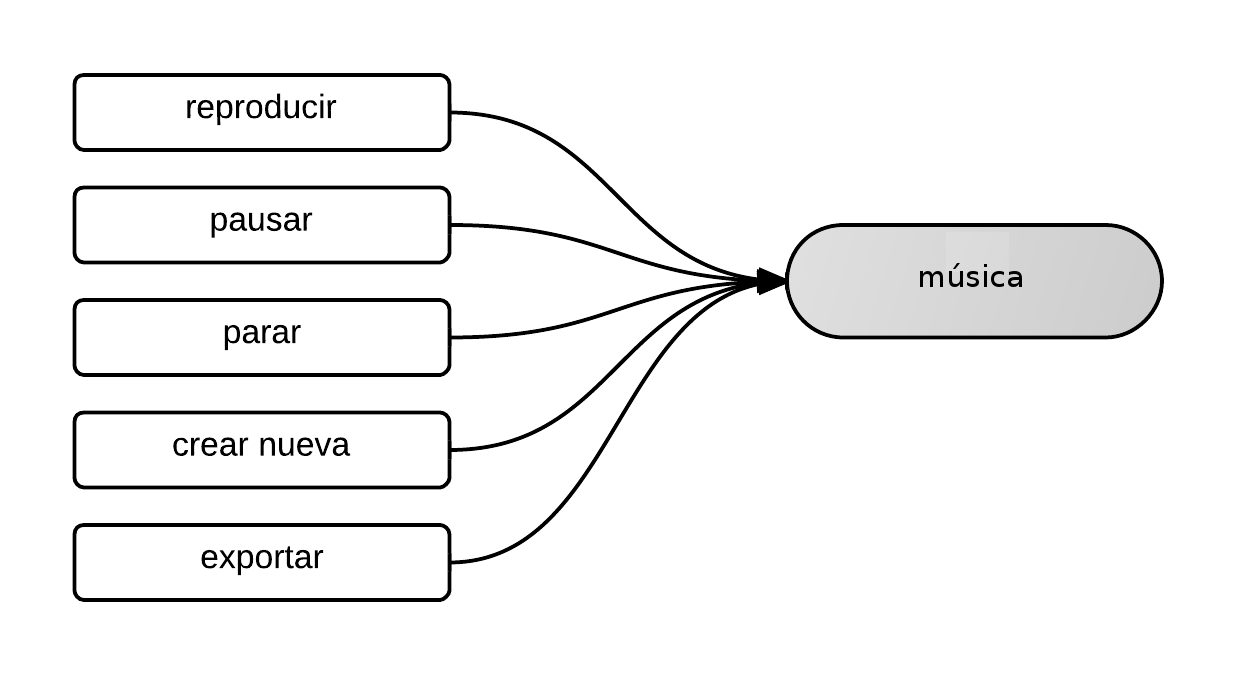
\includegraphics[width=0.5\textwidth]{./graphics/cmd-musica.png}
\caption{Comandos para reproducir, pausar, parar, exportar y crear una m\'usica}
\label{figure:cmd-crear-musica}
\end{figure}

En la figura~\ref{figure:cmd-crear-musica} se pueden observar los comandos m\'as b\'asicos
de la aplicaci\'on, explicados a continuaci\'on:

\begin{itemize}
\item \emph{reproducir m\'usica}: permite reproducir la m\'usica creada.
\item \emph{pausar m\'usica}: permite pausar la reproducci\'on actual dejando la l{\'\i}nea de reproducci\'on en el
punto de pausa.
\item \emph{parar m\'usica}: permite parar la reproducci\'on actual y ubica la l{\'\i}nea de reproducci\'on al inicio de
la m\'usica.
\item \emph{crear nueva m\'usica}:  permite crear una nueva composici\'on, dejando como resultado una
partitura en blanco.
\item \emph{exportar m\'usica}: permite guardar la m\'usica creada en un archivo para que reproducirse en un
reproductor multimedia.
\end{itemize}

\begin{figure}[H]
\begin{minipage}[b]{0.5\linewidth}
\centering
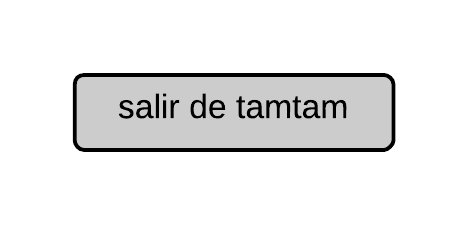
\includegraphics[width=0.6\linewidth]{./graphics/salir.png}
\caption{Comando para salir de la aplicaci\'on}
\label{figure:cmd-salir}
\end{minipage}
\quad
\begin{minipage}[b]{0.5\linewidth}
\centering
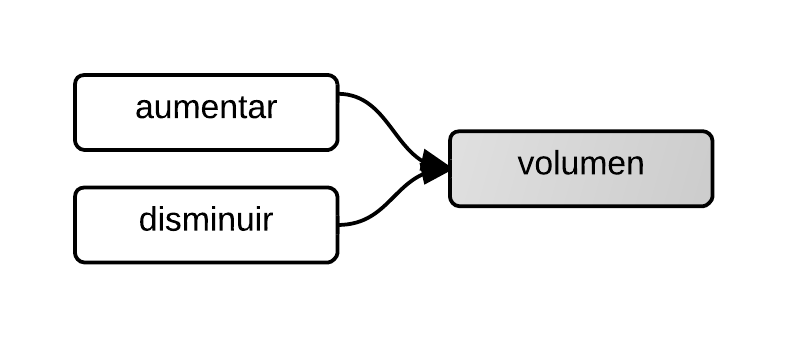
\includegraphics[width=0.6\linewidth]{./graphics/cmd-vol.png}
\caption{Comandos para aumentar/disminuir el volumen general}
\label{figure:cmd-vol}
\end{minipage}
\end{figure}

El comando de la figura~\ref{figure:cmd-salir} permite salir de \emph{TamTam Listens}, basta con decir
``salir de tamtam''. Por otro lado, los comandos de la figura~\ref{figure:cmd-vol}
y~\ref{figure:cmd-tempo} permiten controlar, respectivamente, el volumen y tempo general de la aplicaci\'on. Por ejemplo: ``aumentar volumen'', ``disminuir tempo''.

\begin{figure}[H]
\begin{minipage}[b]{0.5\linewidth}
\centering
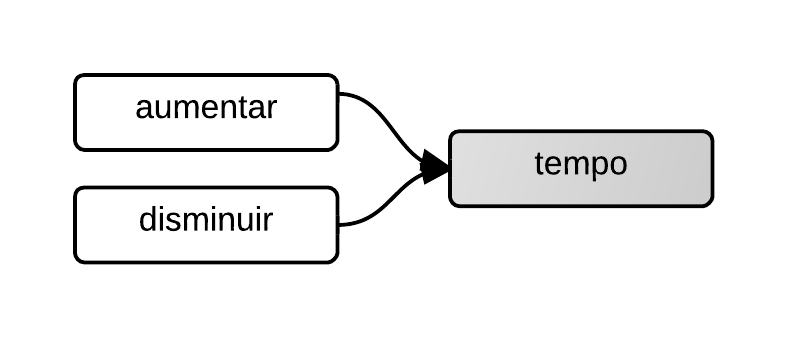
\includegraphics[width=0.6\linewidth]{./graphics/cmd-tempo.png}
\caption{Comandos para aumentar/disminuir el tempo general de al aplicaci\'on}
\label{figure:cmd-tempo}
\end{minipage}
\quad
\begin{minipage}[b]{0.5\linewidth}
\centering
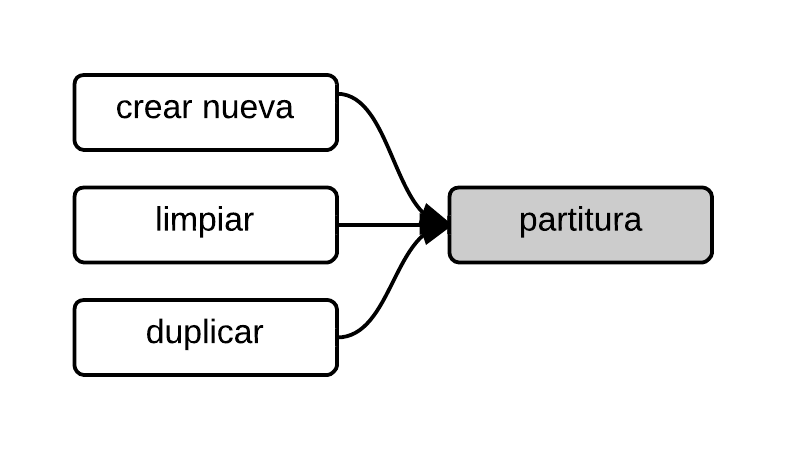
\includegraphics[width=0.6\linewidth]{./graphics/partitura-1.png}
\caption{Comandos para crear, limpiar y duplicar la partitura actual}
\label{figure:cmd-partitura-1}
\end{minipage}
\end{figure}

Los comandos de las figuras~\ref{figure:cmd-partitura-1} y~\ref{figure:cmd-partitura-2} afectan a
la partitura actual, como se explican a continuaci\'on:

\begin{itemize}
    \item \emph{crear nueva  partitura}:  permite crear una nueva partitura en blanco. Utilizaci\'on, 
    ``crear nueva partitura''.
    \item \emph{limpiar  partitura}: permite limpiar el contenido de la partitura actual, es decir, 
    borrar todas las notas. Utilizaci\'on, ``limpiar partitura''.
    \item \emph{duplicar partitura}: crea una nueva partitura con el mismo contenido que la partitura 
    actual. Utilizaci\'on, ``duplicar partitura''.
\end{itemize}

\begin{figure}[H]
\begin{minipage}[b]{0.5\linewidth}
\centering
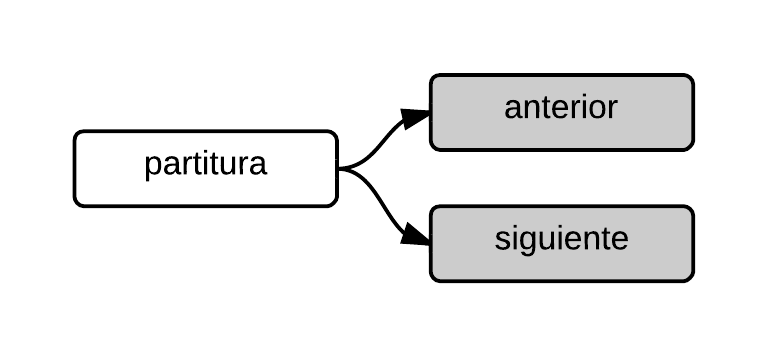
\includegraphics[width=0.6\linewidth]{./graphics/partitura-2.png}
\caption{Comandos para navegar entre partituras}
\label{figure:cmd-partitura-2}
\end{minipage}
\quad
\begin{minipage}[b]{0.5\linewidth}
\centering
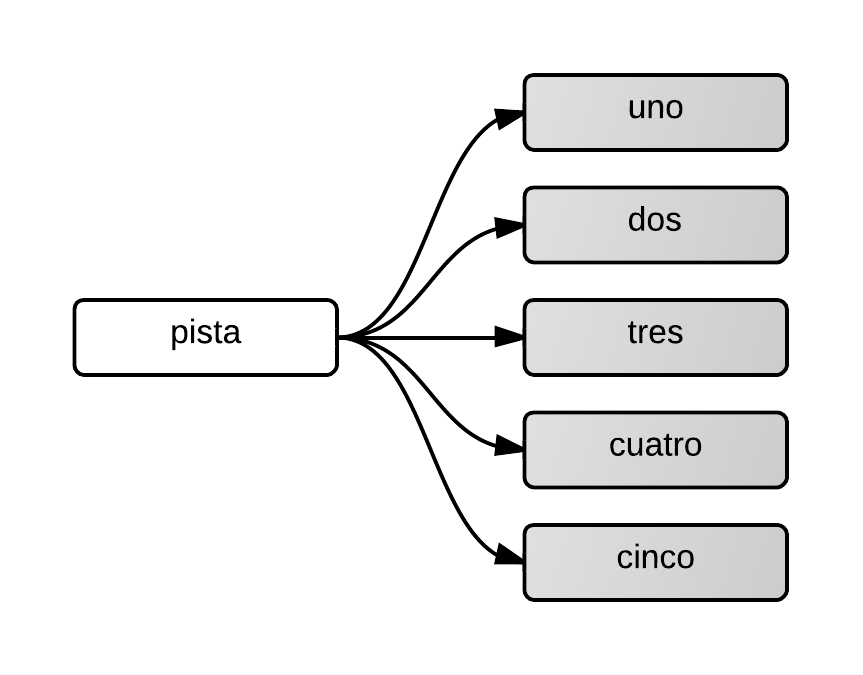
\includegraphics[width=0.6\linewidth]{./graphics/cmd-pista-1.png}
\caption{Comando para ubicarse en una pista}
\label{figure:cmd-pista-1}
\end{minipage}
\end{figure} 

En la figura~\ref{figure:cmd-pista-1} puede apreciarse el comando que permite al usuario ubicarse 
en una pista en particular. Por ejemplo, para ubicarse en la pista tres debe decir “pista tres”. 
Adem\'as de controlar el volumen general de la aplicaci\'on, en 
la figura~\ref{figure:cmd-vol-pista} se pueden ver los comandos para controlar el volumen de una pista en 
particular. Para aumentar el volumen de la pista tres, el usuario debe 
decir ``aumentar volumen de pista tres''.

\begin{figure}[H] 
\begin{minipage}[b]{0.5\linewidth}
\centering
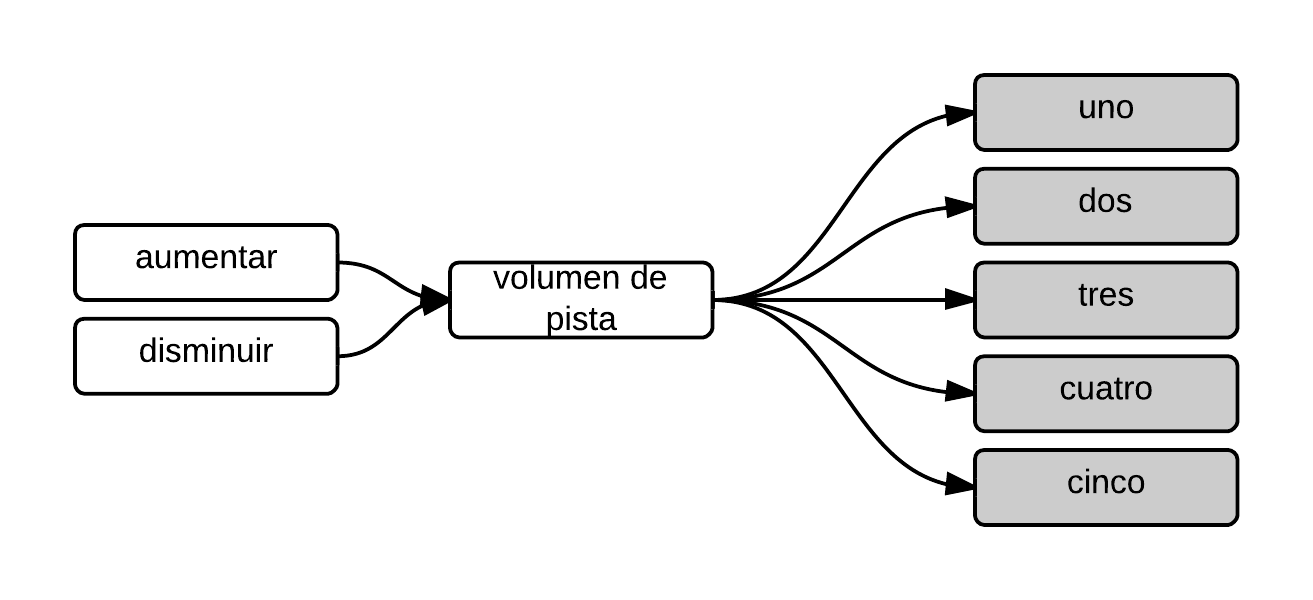
\includegraphics[width=0.8\linewidth]{./graphics/vol-pista.png}
\caption{Comandos para aumentar/disminuir el volumen de una pista en particular}
\label{figure:cmd-vol-pista}
\end{minipage}
\quad
\begin{minipage}[b]{0.5\linewidth}
\centering
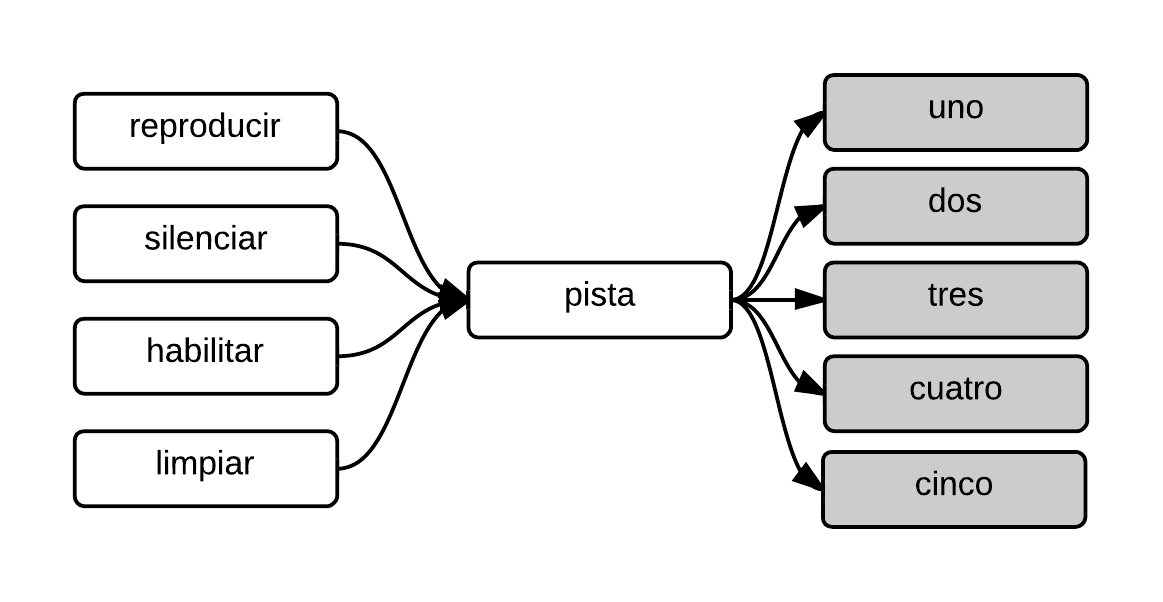
\includegraphics[width=0.9\linewidth]{./graphics/rep-pista.png}
\caption{Comandos para reproducir, silenciar, habilitar y limpiar una pista en particular}
\label{figure:cmd-rep-pista}
\end{minipage}
\end{figure}

Los comandos de la figura~\ref{figure:cmd-rep-pista} permiten: reproducir, silenciar, habilitar y limpiar el contenido de una
pista en particular. Por ejemplo, para reproducir las notas de la pista uno, el usuario debe decir ``reproducir pista uno''. 
Para poder generar distintos tipos de sonidos con \emph{TamTam Listens}, los usuarios de pueden asignar
instrumentos a cada una de las pistas de
la aplicaci\'on, \'esto se puede realizar con los comandos de la figura~\ref{figure:cmd-inst-p1-4} y~\ref{figure:cmd-inst-p5}. Para
asignar el piano a la pista dos, basta con decir ``piano en pista dos''.


\begin{figure}[H]
\centering
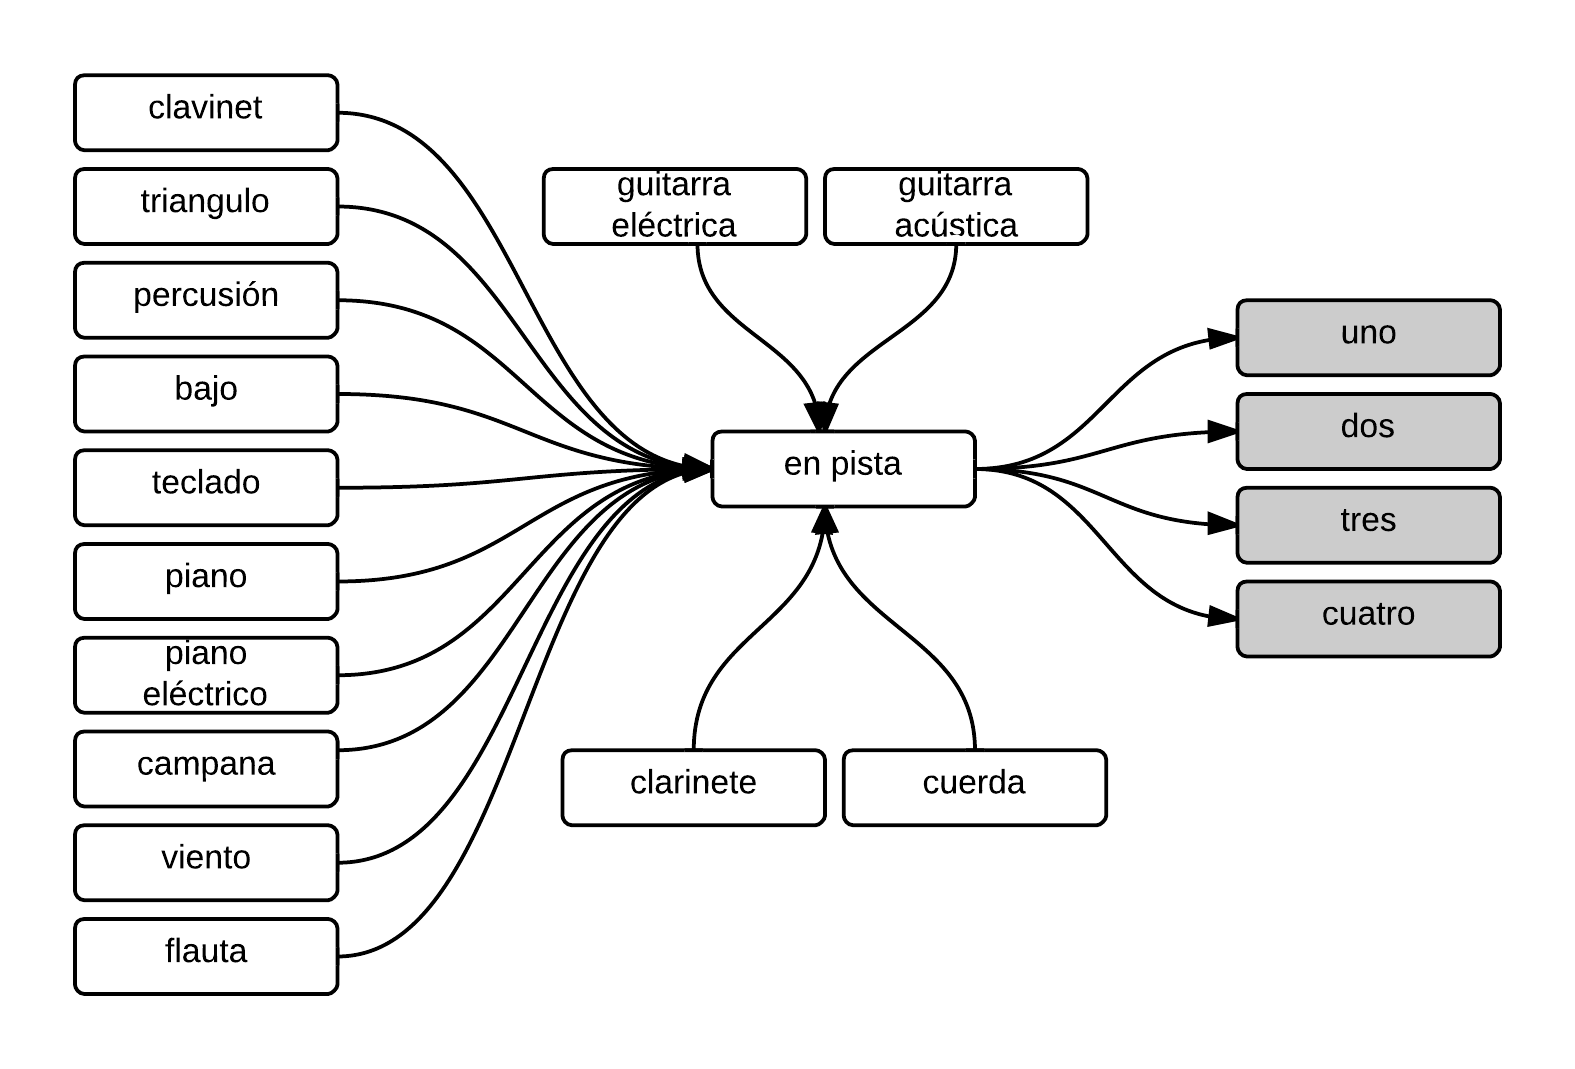
\includegraphics[width=0.8\textwidth]{./graphics/inst-p1-4.png}
\caption{Selecci\'on de instrumento para pistas del uno al cuatro}
\label{figure:cmd-inst-p1-4}
\end{figure}

\begin{figure}[H] 
\begin{minipage}[b]{0.5\linewidth}
\centering
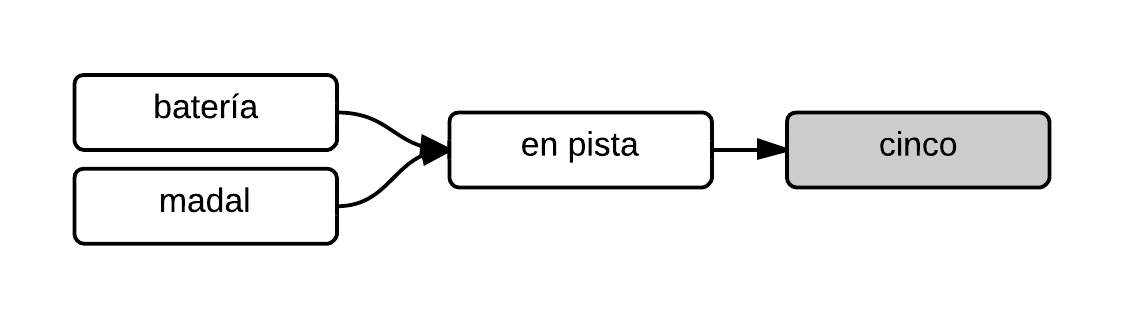
\includegraphics[width=1\linewidth]{./graphics/inst-p5.png}
\caption{Selecci\'on de instrumento para la pista cinco}
\label{figure:cmd-inst-p5}
\end{minipage}
\quad
\begin{minipage}[b]{0.5\linewidth}
\centering
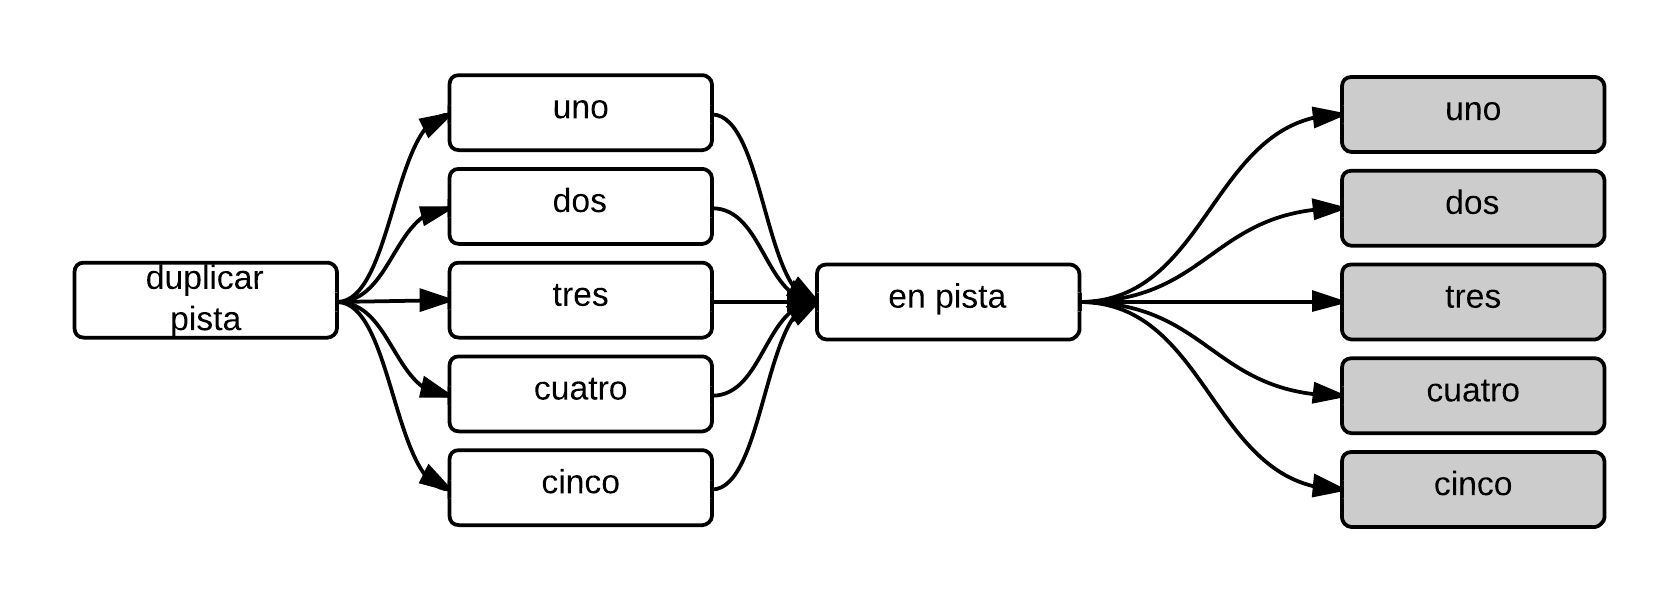
\includegraphics[width=1\linewidth]{./graphics/dup-pista.png}
\caption{Comando para duplicar las notas de una pista en otra}
\label{figure:cmd-dup-pista}
\end{minipage}
\end{figure}

Generalmente las composiciones presentan cierta secuencia de notas que se repiten para varios 
instrumentos. El comando de la figura \ref{figure:cmd-dup-pista} permite duplicar el contenido, 
es decir las notas, de una pista en otra. Por ejemplo, 
``duplicar pista uno en pista dos'' permite duplicar las notas de la pista uno en la pista dos.

\subsubsection{Comandos de Pista} 

Este comando ubica al usuario dentro de una pista en particular. Por lo tanto, se debe
seleccionar una pista para poder utilizar este comando.

\begin{figure}[H] 
\centering
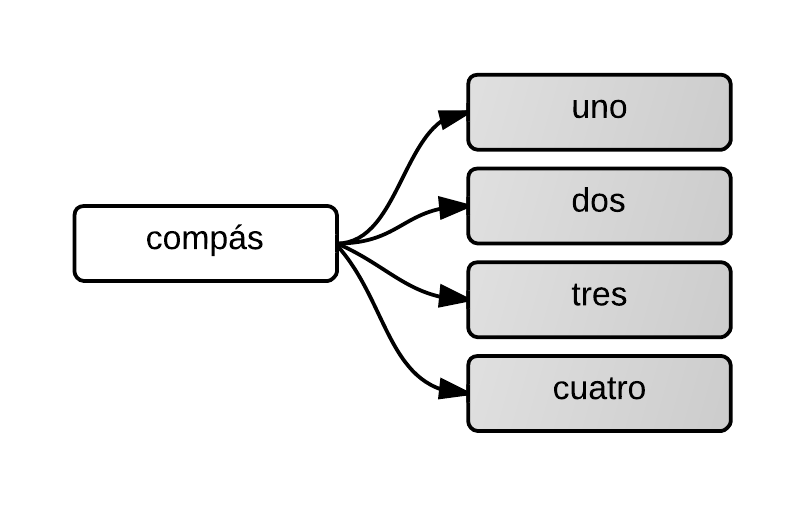
\includegraphics[width=0.4\linewidth]{./graphics/cmd-compas.png}
\caption{Comando para ubicarse en un comp\'as}
\label{figure:cmd-compas}
\quad
\end{figure}

\subsubsection{Comandos de Comp\'as}

Estos comandos son muy importantes para la aplicaci\'on ya que permiten crear, modificar, 
eliminar las notas musicales. El comando de la figura~\ref{figure:cmd-crear-nota} permite crear notas en el  
comp\'as actual, por ejemplo ``crear nota do'' crea la nota do en el comp\'as previamente seleccionado. Por otro lado, en la figura~\ref{figure:cmd-tiempo-compas} 
se muestra el comando que permite al usuario ubicarse en un  
tiempo en espec\'ifico dentro del comp\'as actual. Esto es \'util para crear una nota a partir de ese punto o 
para seleccionar una nota que se encuentre en ese tiempo.

\begin{figure}[H]
\begin{minipage}[b]{0.5\linewidth}
\centering
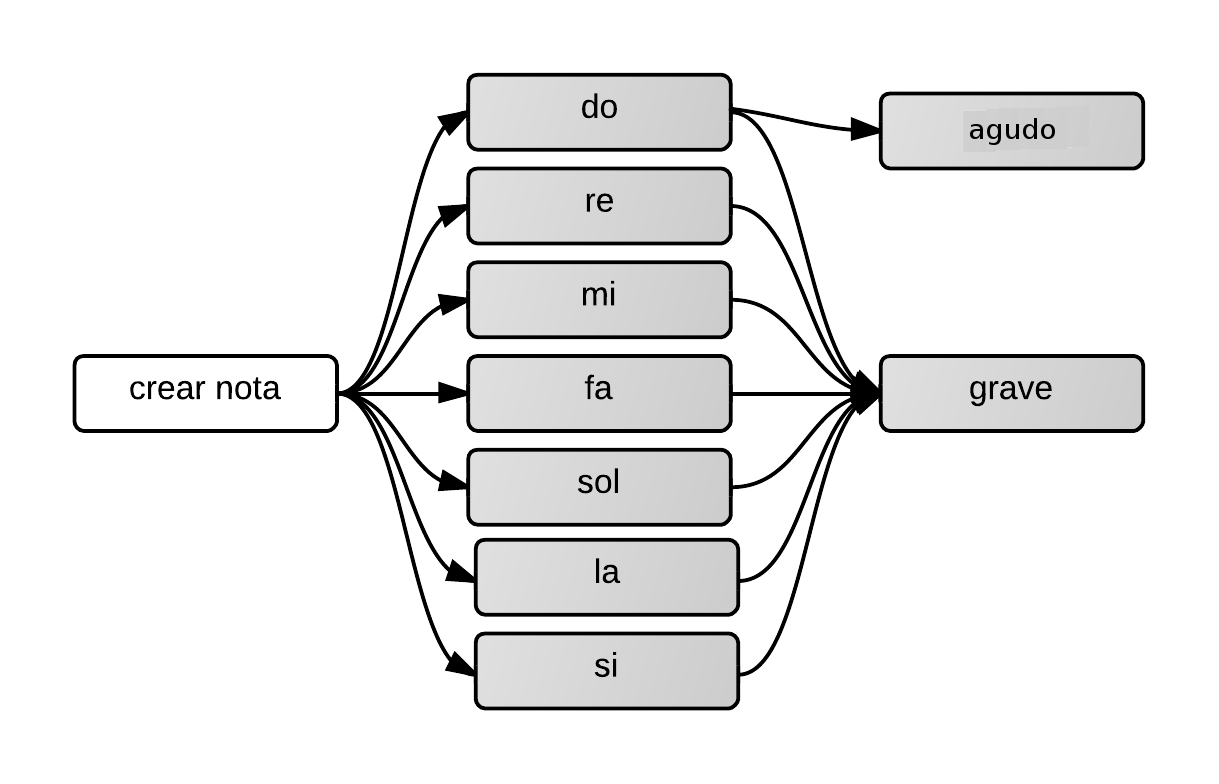
\includegraphics[width=1\linewidth]{./graphics/cmd-crear-nota.png}
\caption{Comando para crear una nota}
\label{figure:cmd-crear-nota}
\end{minipage}
\quad
\begin{minipage}[b]{0.5\linewidth}
\centering
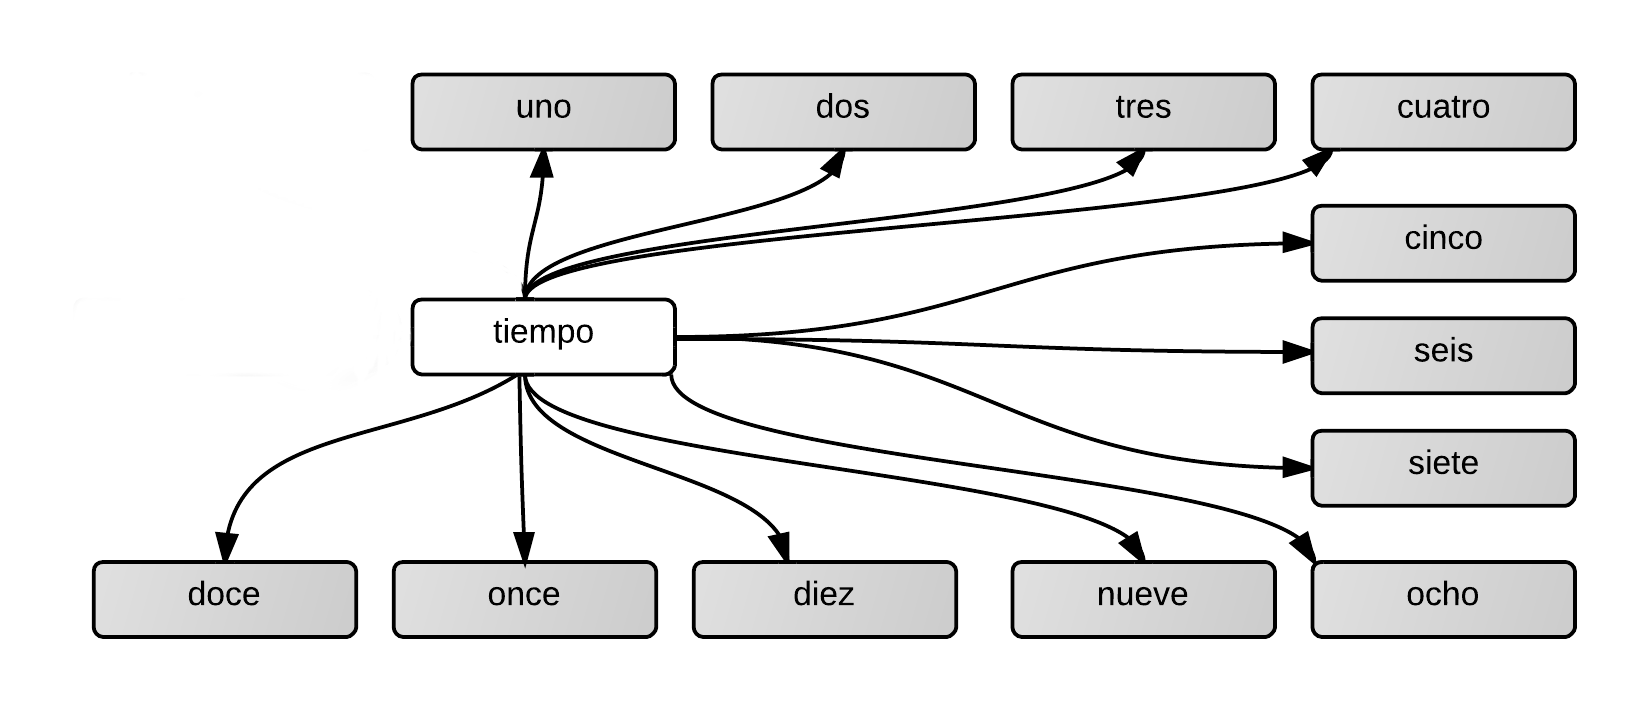
\includegraphics[width=1.1\linewidth]{./graphics/cmd-tiempo-compas.png}
\caption{Comando para ubicarse en un tiempo dado, dentro de un comp\'as}
\label{figure:cmd-tiempo-compas}
\end{minipage}
\end{figure}

As\'i como puede duplicarse notas de una pista a otra, tambi\'en puede duplicarse una nota de un comp\'as a otro utilizando el comando
de la figura~\ref{figure:cmd-dup-nota}, por ejemplo ``duplicar en pista uno compas dos'' permite duplicar una nota en el segundo comp\'as de la pista 
uno. Para poder eliminar una nota, previamente seleccionada, el usuario debe utilizar el comando
de la figura~\ref{figure:cmd-del-nota}.

\begin{figure}[H]
\begin{minipage}[b]{0.5\linewidth}
\centering
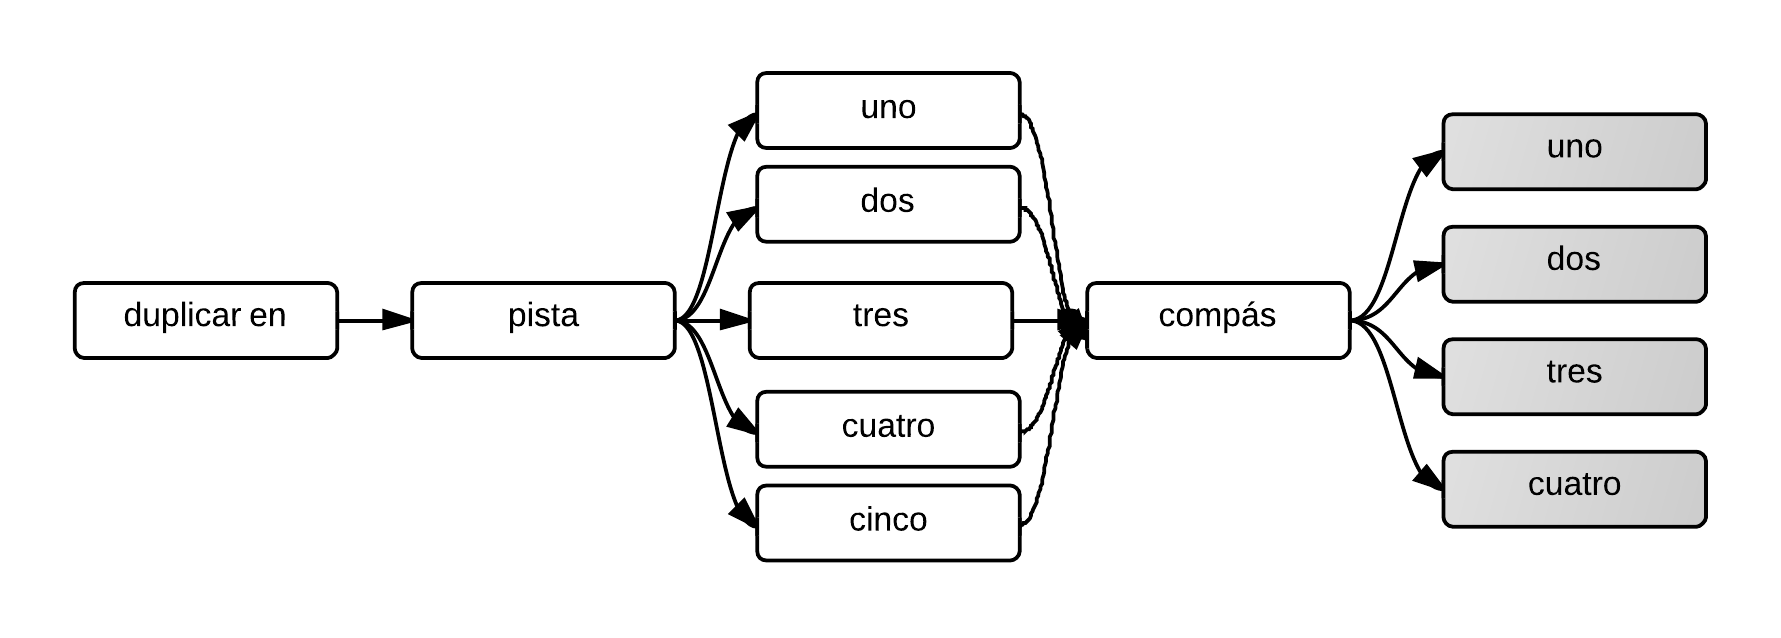
\includegraphics[width=1.2\linewidth]{./graphics/cmd-dup-nota.png}
\caption{Comando para duplicar una nota previamente seleccionada}
\label{figure:cmd-dup-nota}
\end{minipage}
\quad
\begin{minipage}[b]{0.5\linewidth}
\centering
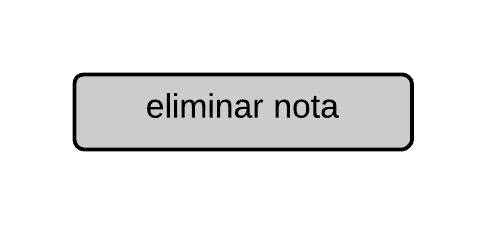
\includegraphics[width=0.5\linewidth]{./graphics/del-note.png}
\caption{Comando para eliminar un nota previamente seleccionada}
\label{figure:cmd-del-nota}
\end{minipage}
\end{figure}

En la figura~\ref{figure:cmd-dur} se pude observar el comando que permite modificar la duraci\'on de 
una nota inmediatamente despu\'es de haberla creado o una nota previamente seleccionada. Finalmente, el comando
presentado en la figura~\ref{figure:cmd-note-tiempo} permite modificar el tiempo en el que inicia la 
nota inmediatamente despu\'es de haberla creado o una nota previamente seleccionada.

\begin{figure}[H]
\begin{minipage}[b]{0.5\linewidth}
\centering
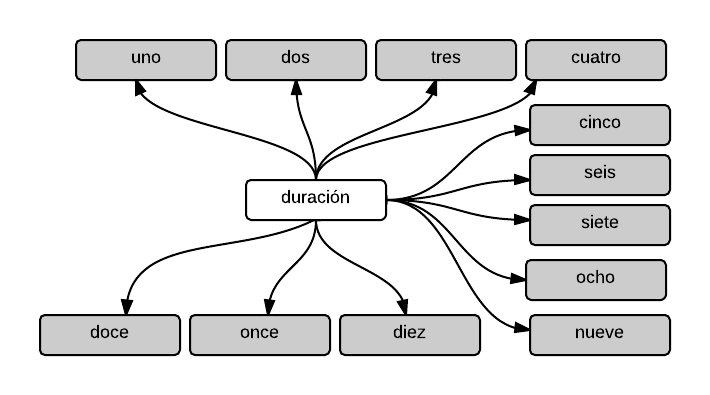
\includegraphics[width=0.9\linewidth]{./graphics/cmd-dur.png}
\caption{Comando que permite configurar la duraci\'on de una nota}
\label{figure:cmd-dur}
\end{minipage}
\quad
\begin{minipage}[b]{0.5\linewidth}
\centering
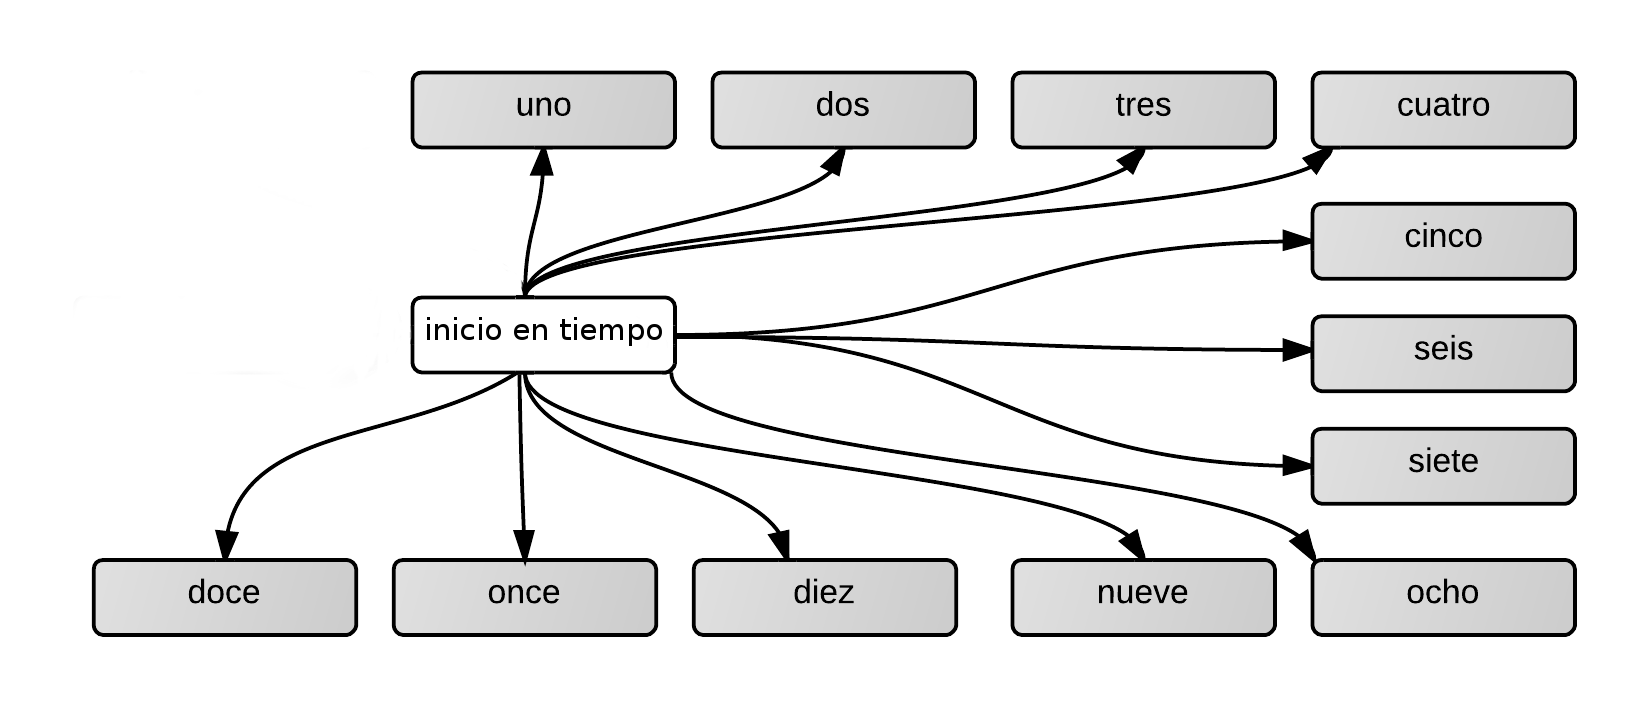
\includegraphics[width=1.1\linewidth]{./graphics/cmd-note-tiempo.png}
\caption{Comando que permite configurar el inicio de una nota dentro del comp\'as}
\label{figure:cmd-note-tiempo}
\end{minipage}
\end{figure}
\section{Tecnolog\'ia a Utilizar}
\label{sec:tecnologia-utilizada}
Para implementar el reconocimiento  de comandos de voz necesario para \foreign{TamTam Listens}, 
se utilizan los proyectos de c\'odigo abierto \emph{Voxforge} \cite{Voxforge} y 
\emph{PocketSphinx} \cite{PocketSphinxHomePage}. 

\subsection{Voxforge}
\label{sec:voxforge-solucion}

\foreign{Voxforge} es un proyecto que busca recopilar grabaciones de voz de modo a crear 
y ofrecer varios corpus de habla bajo una licencia que permita su libre utilizaci\'on. 

A partir de estos corpus, es posible construir modelos ac\'usticos para su uso con motores de 
reconocimiento del habla de c\'odigo abierto, como \foreign{Pocketsphinx}.

\foreign{Voxforge} cuenta con grabaciones en diferentes idiomas, entre ellos ingĺ\'es, franc\'es, 
alem\'an y espa\~nol.


\subsection{PocketSphinx}
\label{sec:pocketsphinx-solucion}

\emph{PocketSphinx} es un motor de reconocimiento del habla orientado a la optimizaci\'on del 
rendimiento y la portabilidad. Es la librería utilizada para la implementaci\'on de la interfaz 
operable a trav\'es de la voz.

Uno de los objetivos espec\'ificos de este trabajo es aplicar y contrastar en la pr\'actica
los conocimientos te\'oricos adquiridos. Como se indica en la secci\'on~\ref{sec:librerias}, 
una librer\'ia requiere conocimiento t\'ecnico espec\'ifico del \'area, adem\'as de
permitir al programador manipular los distintos componentes del proceso de reconocimiento del habla.
Por este motivo, una librer\'ia se considera la herramienta m\'as adecuada para cumplir el objetivo
mencionado anteriormente.

A continuaci\'on se presentan los motivos t\'ecnicos que determinaron la elecci\'on de esta librer\'ia:

\begin{itemize}
    \item \emph{PocketSphinx} est\'a orientada a la optimizaci\'on del rendimiento, resultando adecuada 
    para sistemas con recursos limitados, como la computadora \emph{XO}.
    \item La librer\'ia es un proyecto de c\'odigo abierto, por lo tanto se cumple la metodolog\'ia 
    de trabajo adoptada.
    \item \emph{PocketSphinx} ofrece soporte \emph{offline}, lo cual permite su utilizaci\'on en ambientes
    sin conexi\'on a internet, como ocurre frecuentemente con las \emph{XO}.
    \item Existen \foreign{bindings} para el lenguaje de programaci\'on Python, lo cual hace muy 
    sencilla la tarea de utilizar la librer\'ia desde el c\'odigo Python.
\end{itemize}

\section{Descripci\'on de la Implementaci\'on}
\label{sec:descripcion-implementacion}

En esta secci\'on se describen los detalles de la implementaci\'on de \foreign{TamTam Listens}.
Esto incluye la arquitectura y los componentes propios del sistema de reconocimiento del habla
los cuales, en conjunto con las herramientas mencionadas en las secciones anteriores, hacen posible
el funcionamiento de la interfaz mediante voz. 

\subsection{Arquitectura de TamTam Listens}
\label{sec:arquitectura-solucion}

La figura~\ref{figure:tamtam-listens-arq} muestra la arquitectura b\'asica de \emph{TamTam Listens}. Se 
pueden observar los componentes que forman parte de la soluci\'on desarrollada.

\begin{figure}[H] 
\centering

\includegraphics[width=0.7\textwidth]{./graphics/tamtam-listens-arq.png}
\caption{Arquitectura b\'asica de \emph{TamTam Listens}}
\label{figure:tamtam-listens-arq}
\end{figure}

Como sugiere la figura~\ref{figure:tamtam-listens-arq}, \emph{TamTam Listens} a\~nade soporte 
de reconocimiento del habla a \emph{TamTam Edit} utilizando la librer\'ia \emph{PocketSphinx}.
A favor de una soluci\'on modular, el reconocimiento de comandos de voz de \emph{PocketSphinx} 
es expuesto como como un  servicio del sistema, a trav\'es de llamadas a \emph{D-Bus}\cite{Dbus2013},
el cual es un mecanismo para comunicaci\'on entre procesos de Linux\footnote{Linux es un sistema operativo
cuyo \foreign{kernel} y paquetes de software son desarrollados bajo el modelo de c\'odigo abierto\cite{LinuxGuideCert}}.

\emph{TamTam Listens} consume como un servicio el reconocimiento del habla expuesto a trav\'es de 
\emph{D-Bus}, utilizando un protocolo de paso de mensajes.

La arquitectura propuesta, implementada como parte de \emph{TamTam Listens}, favorece la modularidad
y facilita la reutilizaci\'on de la soluci\'on para otros proyectos de caracter{\'\i}sticas similares.

La figura \ref{figure:tamtam-listens-proceso} representa el proceso completo de interacci\'on entre el
usuario y \emph{TamTam Listens}, el cual est\'a compuesto por los siguientes pasos:

\begin{itemize}
  \item Inicialmente, el usuario pronuncia un comando de voz que se registra mediante el micr\'ofono de
  la computadora donde se ejecuta \emph{TamTam Listens}.
  \item La entrada sonora es procesada por \emph{Pocketsphinx}, pasando por las etapas del proceso del
  reconocimiento del habla descrito en el cap{\'\i}tulo \ref{sec:proceso}. El resultado es una cadena de
  texto correspondiente al comando reconocido.
  \item La salida de \emph{Pocketsphinx} es registrada por su proceso padre, un demonio que expone
  una se\~nal \emph{D-Bus}.
  El demonio \emph{D-Bus}, a su vez, env{\'\i}a el resultado a todos los procesos registrados 
  a la se\~nal.
  En este caso, el \'unico proceso que recibe el resultado es \emph{TamTam Listens}.
  \item Al recibir el comando reconocido, \emph{TamTam Listens} ejecuta la acci\'on correspondiente de
  acuerdo a un conjunto de reglas definidas por la aplicaci\'on.
\end{itemize}

\begin{figure}[H] 
\centering
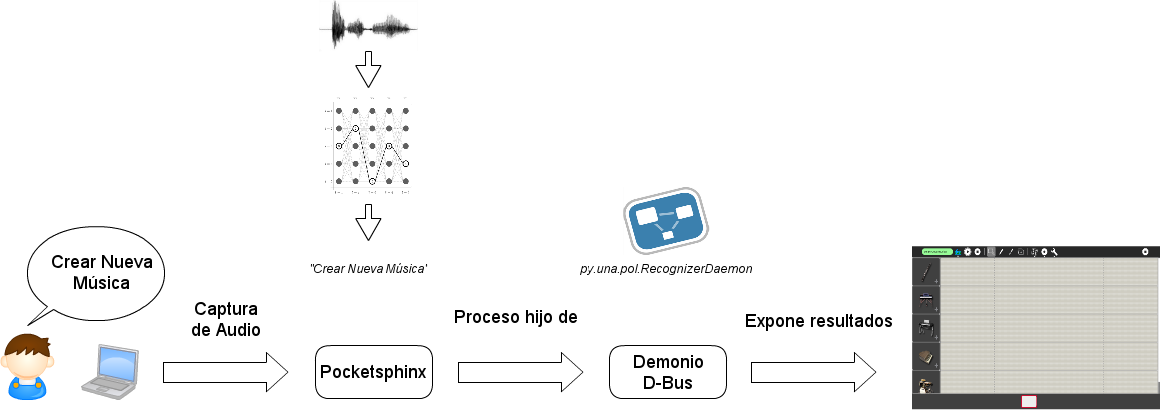
\includegraphics[width=1.0\textwidth]{./graphics/tamtam-proceso.png}
\caption{Implementación de una interfaz mediante voz del usuario para \emph{TamTam Listens}}
\label{figure:tamtam-listens-proceso}
\end{figure}

\subsection{Proceso del Reconocimiento del Habla}
\label{sec:proceso-solucion}

\foreign{PocketSphinx} implementa el proceso del reconocimiento del habla basado en el enfoque 
estad{\'\i}stico, el cual se present\'o en el cap{\'\i}tulo~\ref{sec:proceso}. La librer{\'\i}a incluye
los diferentes algoritmos necesarios para las fases del proceso.

\begin{figure}[H] 
\centering
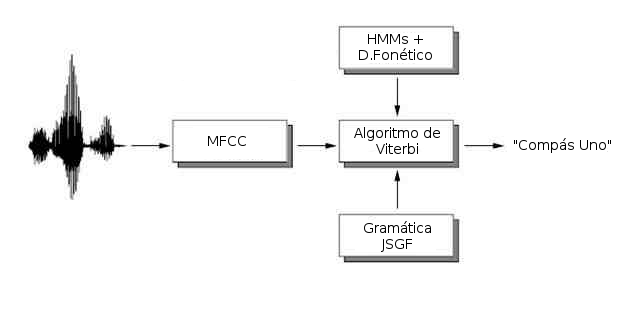
\includegraphics[width=0.8\textwidth]{./graphics/pocketsphinx.png}
\caption{Reconocimiento del habla mediante PocketSphinx. Gr\'afico basado en \cite{VerenichASR}.}
\label{figure:proceso-pocketsphinx}
\end{figure}

Como conjunto de caracter{\'\i}sticas espectrales, \foreign{Pocketsphinx} utiliza los coeficientes
espectrales en las frecuencias de mel (MFCC por sus siglas en ingl\'es).

En los \gls{hmm} del modelo ac\'ustico, utiliza mezclas Gaussianas para definir las probabilidades de 
transici\'on entre estados. El diccionario fon\'etico debe ser definido por el desarrollador.

Aunque \foreign{PocketSphinx} soporta modelos de lenguaje basados en n-gramas, para este trabajo 
se utiliza un modelo de lenguaje basado en gram\'atica. Esto se debe a la simpleza del lenguaje y a la 
falta de datos de entrenamiento para un modelo estad{\'\i}stico del mismo.

Como decodificador se utiliza el algoritmo de Viterbi, haciendo uso de la t\'ecnica de b\'usqueda en haz
para reducir el espacio de b\'usqueda.

Para hacer posible el reconocimiento del habla debe definirse el vocabulario que forma parte del 
dominio de la aplicaci\'on, su pronunciaci\'on y el conjunto de oraciones (en este caso, comandos 
v\'alidos) soportados por la aplicaci\'on. En otras palabras, \emph{Pocketsphinx} requiere un
modelo ac\'ustico y un modelo de lenguaje para funcionar.

\subsection{Modelo Ac\'ustico}
\label{sec:acustico-solucion}

El modelo ac\'ustico utilizado tiene como base las grabaciones de \foreign{Voxforge} en idioma espa\~nol,
y se encuentra disponible entre los recursos del proyecto \foreign{Pocketsphinx} para su utilizaci\'on
con el motor de reconocimiento del habla.

El diccionario fon\'etico define la secuencia de fonemas de cada palabra del lenguaje.
Este diccionario es utilizado por \emph{PocketSphinx} para asociar los fonemas reconocidos por
el modelo ac\'ustico a palabras v\'alidas del dominio de la aplicaci\'on.
En la figura~\ref{figure:fragmento-dic} se puede observar un fragmento del diccionario fon\'etico
utilizado por \emph{TamTam Listens}.

\lstset{
  basicstyle=\scriptsize,        % the size of the fonts that are used for the code
  breakatwhitespace=false,         % sets if automatic breaks should only happen at whitespace
  frame=single,                    % adds a frame around the code
  language=Octave,                 % the language of the code
  numbersep=5pt,                   % how far the line-numbers are from the code
  showstringspaces=false,          % underline spaces within strings only
  stepnumber=2,                    % the step between two line-numbers. If it's 1, each line will be numbered
  tabsize=2                       % sets default tabsize to 2 spaces
}

\begin{figure}[H]
\begin{lstlisting}
REPRODUCIR RR E P R O D U S I R
PAUSAR P A U S A R
PARAR  P A R A R
GENERAR  J E N E R A R
PARTITURA P A R T I T U R A
SIGUIENTE S I G I E N T E
ANTERIOR A N T E R I O R
\end{lstlisting}
\caption{Fragmento del diccionario fon\'etico utilizado en \emph{Tamtam Listens}.}
\label{figure:fragmento-dic}
\end{figure}

Como se puede observar, el formato del diccionario es bastante simple. Primero se define la palabra y 
a continuaci\'on los fonemas que la componen separados por espacios.
Una vez definidas las palabras de la aplicaci\'on, lo siguiente es determinar si una secuencia de
palabras es o no un comando v\'alido.

\subsection{Modelo de Lenguaje}
\label{sec:lenguaje-solucion}

Para el modelo de lenguaje se utiliza una gram\'atica en formato JSGF \cite{JSGF2000}, la cual permite
definir los comandos soportados por la aplicaci\'on de una manera sencilla.
En la figura~\ref{figure:fragmento-gram} puede observarse un fragmento de la gram\'atica utilizada por 
la aplicaci\'on.

\begin{figure}[H]
\begin{lstlisting}
#JSGF V1.0;
grammar tamtam;

public <tamtam-listens> = <comando> | <pagina> | <pista-a>     | <pista-b>  | 
                          <seleccionar-compas> | <crear-nota>  | <seleccionar-nota> | 
                          <duplicar-nota>      | <borrar-nota> | <volumen> | <tempo> | 
                          <configurar-nota>    | <loop>;

<comando>  = REPRODUCIR MUSICA  | PAUSAR MUSICA   | PARAR MUSICA | GENERAR MUSICA | 
             CREAR NUEVA MUSICA | EXPORTAR MUSICA | SALIR DE TAMTAM;
<pagina>   = ( CREAR NUEVA | DUPLICAR | LIMPIAR ) PARTITURA | PARTITURA <orden>;
<orden>    = ( ANTERIOR | SIGUIENTE );
<loop>     = (COMODIN)+;
\end{lstlisting}
\caption{Fragmento de la gram\'atica utilizada en \emph{Tamtam Listens}.}
\label{figure:fragmento-gram}
\end{figure} 


\subsection{Palabras fuera del Vocabulario}
\label{sec:oov}

La pronunciaci\'on de palabras fuera del vocabulario ocurre frecuentemente en numerosas aplicaciones
del reconocimiento del habla, y es una fuente conocida de errores en el reconocimiento \cite{Bazzi00Modeling}.

De modo a minimizar la cantidad de errores como consecuencia de las palabras fuera del vocabulario,
\foreign{TamTam Listens} integra a su gram\'atica un modelo de palabra gen\'erica. Este componente se
define mediante el no terminal $<loop>$ de la figura \ref{figure:fragmento-gram}.

Un modelo de palabra gen\'erica admite cualquier palabra que pueda pronunciarse, es decir, permite
cualquier secuencia arbitraria de fonemas \cite{Bazzi00Modeling}. 
En el caso de \foreign{TamTam Listens}, el no terminal $<loop>$ corresponde a una o m\'as repeticiones del
terminal $COMODIN$.

A su vez, el terminal $COMODIN$ est\'a asociado a cada uno de los fonemas en el diccionario fon\'etico de
\foreign{TamTam Listens}, como se observa en la figura \ref{figure:fragmento-comodin}.

\begin{figure}[H]
\begin{lstlisting}
COMODIN   A
COMODIN(2)  B
COMODIN(3)  C
COMODIN(4)  CH
COMODIN(5)  D
\end{lstlisting}
\caption{Definici\'on parcial de COMODIN en el diccionario de \emph{Tamtam Listens}.}
\label{figure:fragmento-comodin}
\end{figure}

La combinaci\'on de los componentes presentados en este cap\'itulo hizo posible implementar el motor 
de reconocimiento del habla como servicio de \emph{D-Bus} y as\'i ofrecer \emph{TamTam Listens} como una 
interfaz alternativa a la propuesta por \emph{TamTam Edit}.

En el siguiente cap\'itulo se presenta la evaluaci\'on de la interfaz implementada, teniendo en cuenta 
aspectos t\'ecnicos y funcionales.

